\documentclass{article}
\usepackage[english]{babel}
\usepackage[letterpaper,top=1.7cm,bottom=1.7cm,left=2.2cm,right=2.2cm,marginparwidth=1.75cm]{geometry}
\usepackage{graphicx}
\usepackage[colorlinks=true, allcolors=blue]{hyperref}
\usepackage{url}
\usepackage{array}
\usepackage{amsmath,amssymb,amsfonts}
\usepackage{textcomp}
\usepackage{xcolor}
\usepackage{tabularx}
\usepackage{makecell}
\usepackage{multirow}
\usepackage{booktabs}
\usepackage{subcaption}
\usepackage{float}

\title{CSE621 Spring26 Project 4: Large Language Models for Classification and Clustering}
\author{
Shang Liu, Hanyu Pei \\
\texttt{\small{\{shang.liu, hanyu.pei\}@louisville.edu}} \\
\texttt{\small{Code: \url{https://github.com/liuup/CSE621_project4}}} \\
\texttt{\small{Video: }} \\
}

\begin{document}
\maketitle

\section{Objectives}

This project studies how encoder-based language models, decoder-only language models, and classical text models behave on two standard text mining tasks: supervised classification and unsupervised clustering. Following the project instructions, all experiments use the Hugging Face \texttt{SetFit/bbc-news} dataset and evaluate on its default test split. The dataset contains five balanced BBC news categories: \texttt{business}, \texttt{entertainment}, \texttt{politics}, \texttt{sport}, and \texttt{tech}. Our goals are:

\begin{itemize}
\item compare encoder, decoder, and classical approaches for multi-class document classification,
\item compare encoder-derived and classical text representations for clustering, and
\item analyze the tradeoff between predictive quality and runtime.
\end{itemize}

\section{Dataset}

We use the pre-split \texttt{SetFit/bbc-news} dataset from Hugging Face. The training split contains 1,225 articles and the test split contains 1,000 articles. Because the project instructions explicitly require evaluation on the provided default test split, no custom train/test split was created. Labels were used directly for classification, and only for external evaluation in clustering.

This dataset is a good fit for the project because it is small enough to support repeated model comparison while still containing realistic topical variation. The five classes are semantically related enough that the task is not trivial, but sufficiently distinct that both lexical and semantic methods can be meaningfully compared. That balance makes it possible to see where classical sparse models are still strong and where transformer-based representations provide additional value.

\section{Part 1: Classification}

\subsection{Methodology}

We implemented five required classifier families and, for the classical baseline, evaluated three linear variants.

\paragraph{Encoder frozen-head classifier.}
We used \texttt{bert-base-uncased} as a pretrained encoder. The encoder weights were frozen and only a linear classification head was trained on top of the pooled encoder output. Training used the BBC training split, AdamW, a small validation split, and CUDA acceleration.

This setup was chosen because it matches the requirement to use a pretrained encoder as a frozen layer while keeping the implementation simple and computationally efficient. It also isolates the value of the pretrained representation itself: any performance gain comes primarily from the encoder features rather than from large-scale end-to-end fine-tuning.

\paragraph{Encoder zero-shot classifier.}
We used \texttt{sentence-transformers/all-MiniLM-L6-v2} without task-specific training. Each test article and each label description were embedded into the same space, and prediction was made by cosine-similarity matching.

The label descriptions were written as short natural-language category prompts instead of using bare label strings only. This makes the zero-shot setting slightly more realistic, since the model can align documents against semantic descriptions such as business, politics, or entertainment rather than just arbitrary tokens.

\paragraph{Decoder zero-shot and few-shot classifiers.}
We used \texttt{Qwen/Qwen2.5-1.5B-Instruct}. The initial free-form generation approach was unstable, so the final system scores the five candidate labels directly under the decoder model and chooses the label with the best conditional score. This still follows the project requirement of decoder-based zero-shot and few-shot prompting, but replaces fragile string parsing with label scoring. For few-shot prompting, one training example per class was inserted into the prompt.

This change was important in practice. In early runs, free-form generation often produced incomplete phrases or continuations that were semantically related to the article but not exact labels. Candidate-label scoring avoids this parsing problem and turns the decoder into a more reliable prompted classifier while keeping the experiment faithful to the decoder-only setting.

\paragraph{Classical baselines.}
We used TF-IDF features with three classical classifiers: Logistic Regression, Linear SVM, and Multinomial Naive Bayes. The best classical result is still reported as the main classical baseline, while the other two are included for completeness.

\paragraph{Metrics.}
Following the instructions, all classification models were compared using Accuracy, Precision, Recall, F1-score, and runtime.

All runtimes were measured inside the same codebase and environment so that relative comparisons are meaningful. Encoder and decoder models were run on CUDA, while the classical pipelines were lightweight enough to finish almost immediately on the same machine.

\subsection{Experimental Results \& Analysis}

\begin{table}[H]
\centering
\small
\caption{Classification results on the BBC News test split.}
\label{tab:classification}
\begin{tabular}{lccccc}
\toprule
Model & Accuracy & Precision & Recall & F1 & Runtime (s) \\
\midrule
Encoder frozen head & 0.946 & 0.9464 & 0.946 & 0.9460 & 5.50 \\
Encoder zero-shot & 0.838 & 0.8387 & 0.838 & 0.8363 & 0.41 \\
Decoder zero-shot & 0.687 & 0.8106 & 0.687 & 0.6879 & 36.28 \\
Decoder few-shot & 0.689 & 0.8113 & 0.689 & 0.6764 & 38.42 \\
TF-IDF + Logistic Regression & 0.963 & 0.9632 & 0.963 & 0.9631 & 1.60 \\
TF-IDF + Linear SVM & \textbf{0.965} & \textbf{0.9654} & \textbf{0.965} & \textbf{0.9651} & 0.18 \\
TF-IDF + Naive Bayes & 0.956 & 0.9572 & 0.956 & 0.9559 & 0.16 \\
\bottomrule
\end{tabular}
\end{table}

\begin{figure}[H]
\centering
\begin{subfigure}{0.49\textwidth}
    \centering
    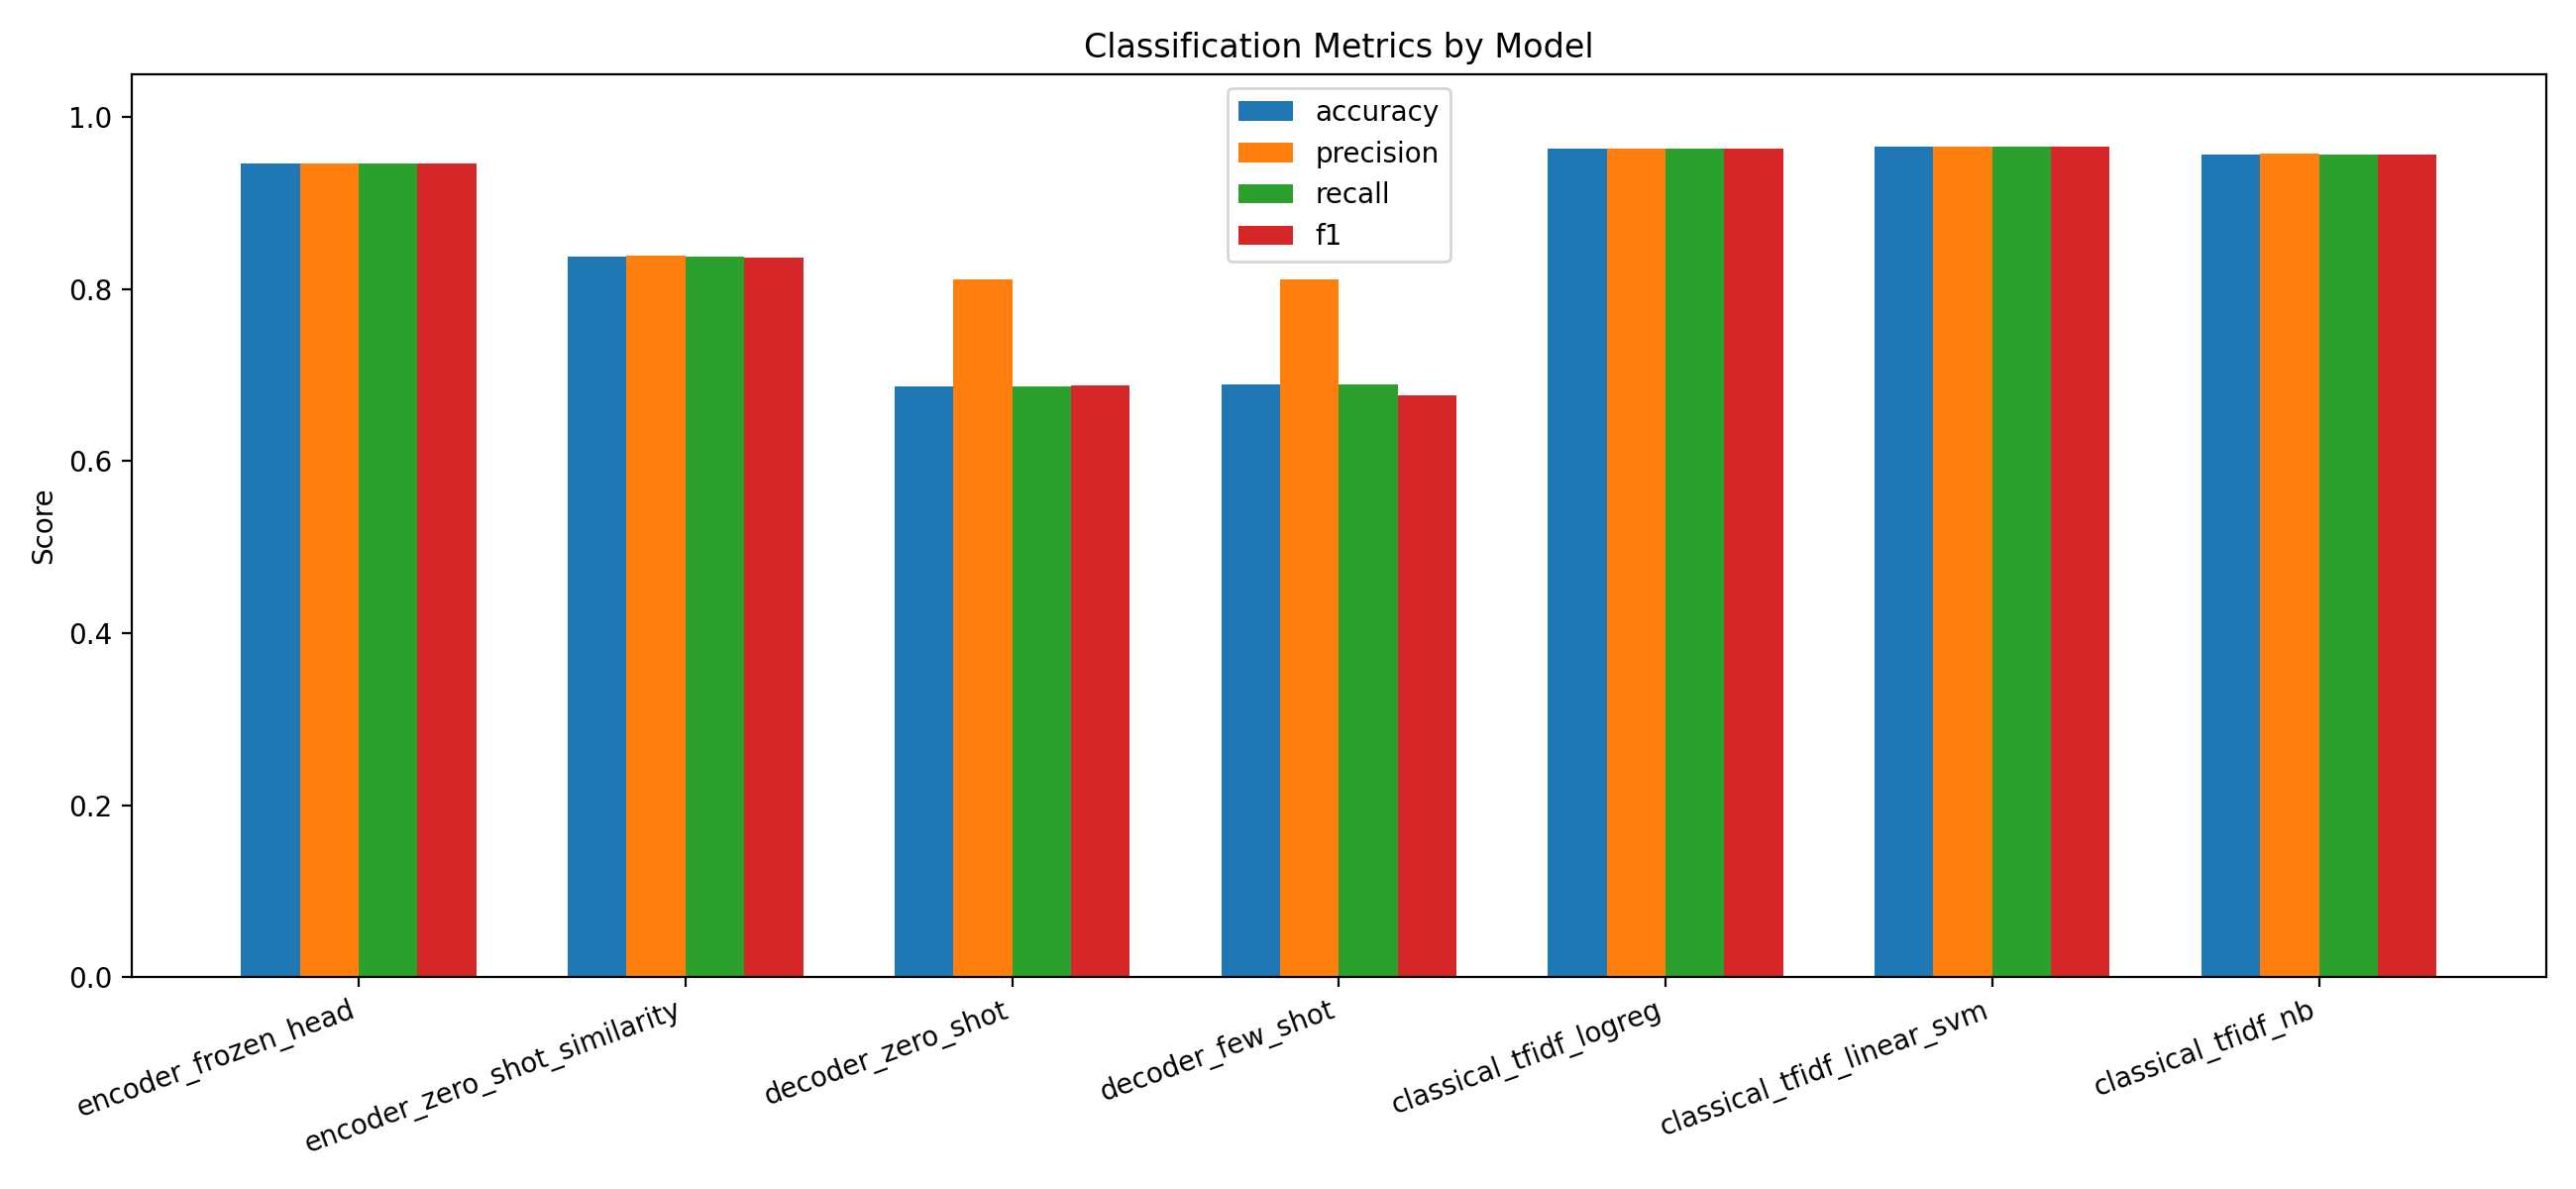
\includegraphics[width=\linewidth]{results_final_all/classification/classification_metrics.png}
    \caption{Classification metrics comparison}
\end{subfigure}
\hfill
\begin{subfigure}{0.49\textwidth}
    \centering
    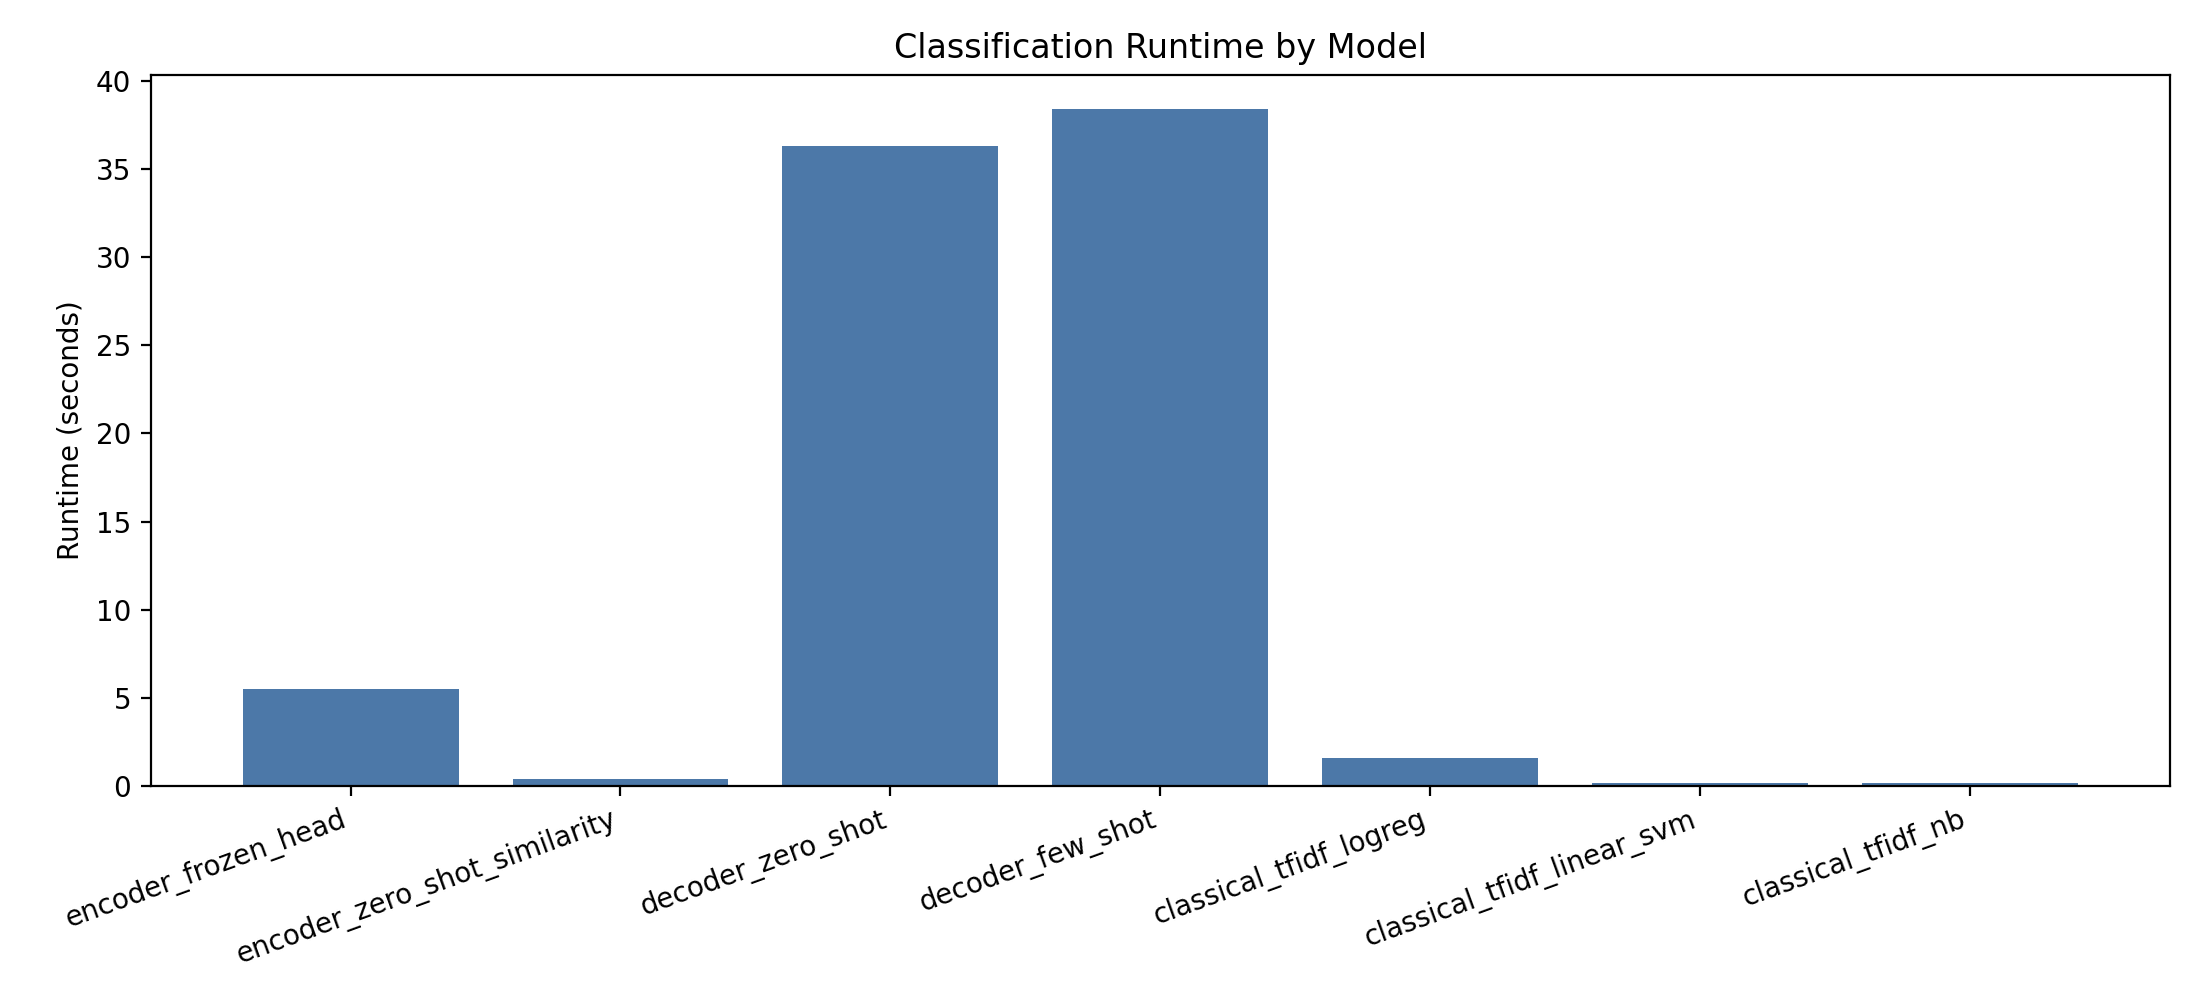
\includegraphics[width=\linewidth]{results_final_all/classification/classification_runtimes.png}
    \caption{Classification runtime comparison}
\end{subfigure}
\caption{Summary plots for Part 1 classification experiments.}
\label{fig:classification-plots}
\end{figure}

The best overall classifier was the TF-IDF + Linear SVM baseline, with 0.965 accuracy and 0.9651 weighted F1. This result is slightly better than the frozen encoder classifier, which reached 0.946 accuracy. On this dataset, the classical linear model benefits from a clean, relatively small label space and category-specific vocabulary. BBC topics such as sport, politics, and entertainment have strong lexical cues, and TF-IDF preserves these cues very effectively.

The encoder frozen-head model was the strongest neural classifier. Its performance shows that pretrained encoder representations transfer very well even when only a shallow head is trained. The encoder zero-shot similarity method performed clearly worse than the trained encoder model but still remained strong at 0.838 accuracy, which is a useful result because it requires no task-specific training.

The decoder models improved substantially after replacing free-form label generation with direct candidate-label scoring. The final decoder zero-shot and few-shot models both reached about 0.69 accuracy, far above the earlier unstable runs. However, they still lag behind encoder and classical models. The decoder is much slower and less calibrated for short-label classification than a frozen encoder or a sparse linear classifier. Few-shot prompting provided only a very small gain in accuracy, suggesting that one example per class was not enough to reshape the label decision boundary strongly.

The runtime comparison is also informative. The strongest classical model is not only the most accurate but also one of the fastest. By contrast, the decoder methods are by far the slowest approaches, yet they still underperform the encoder and classical baselines. This highlights an important practical point: decoder-only prompting is flexible and easy to prototype, but it is not always the most efficient tool for a constrained label-classification problem.

\begin{figure}[H]
\centering
\begin{subfigure}{0.49\textwidth}
    \centering
    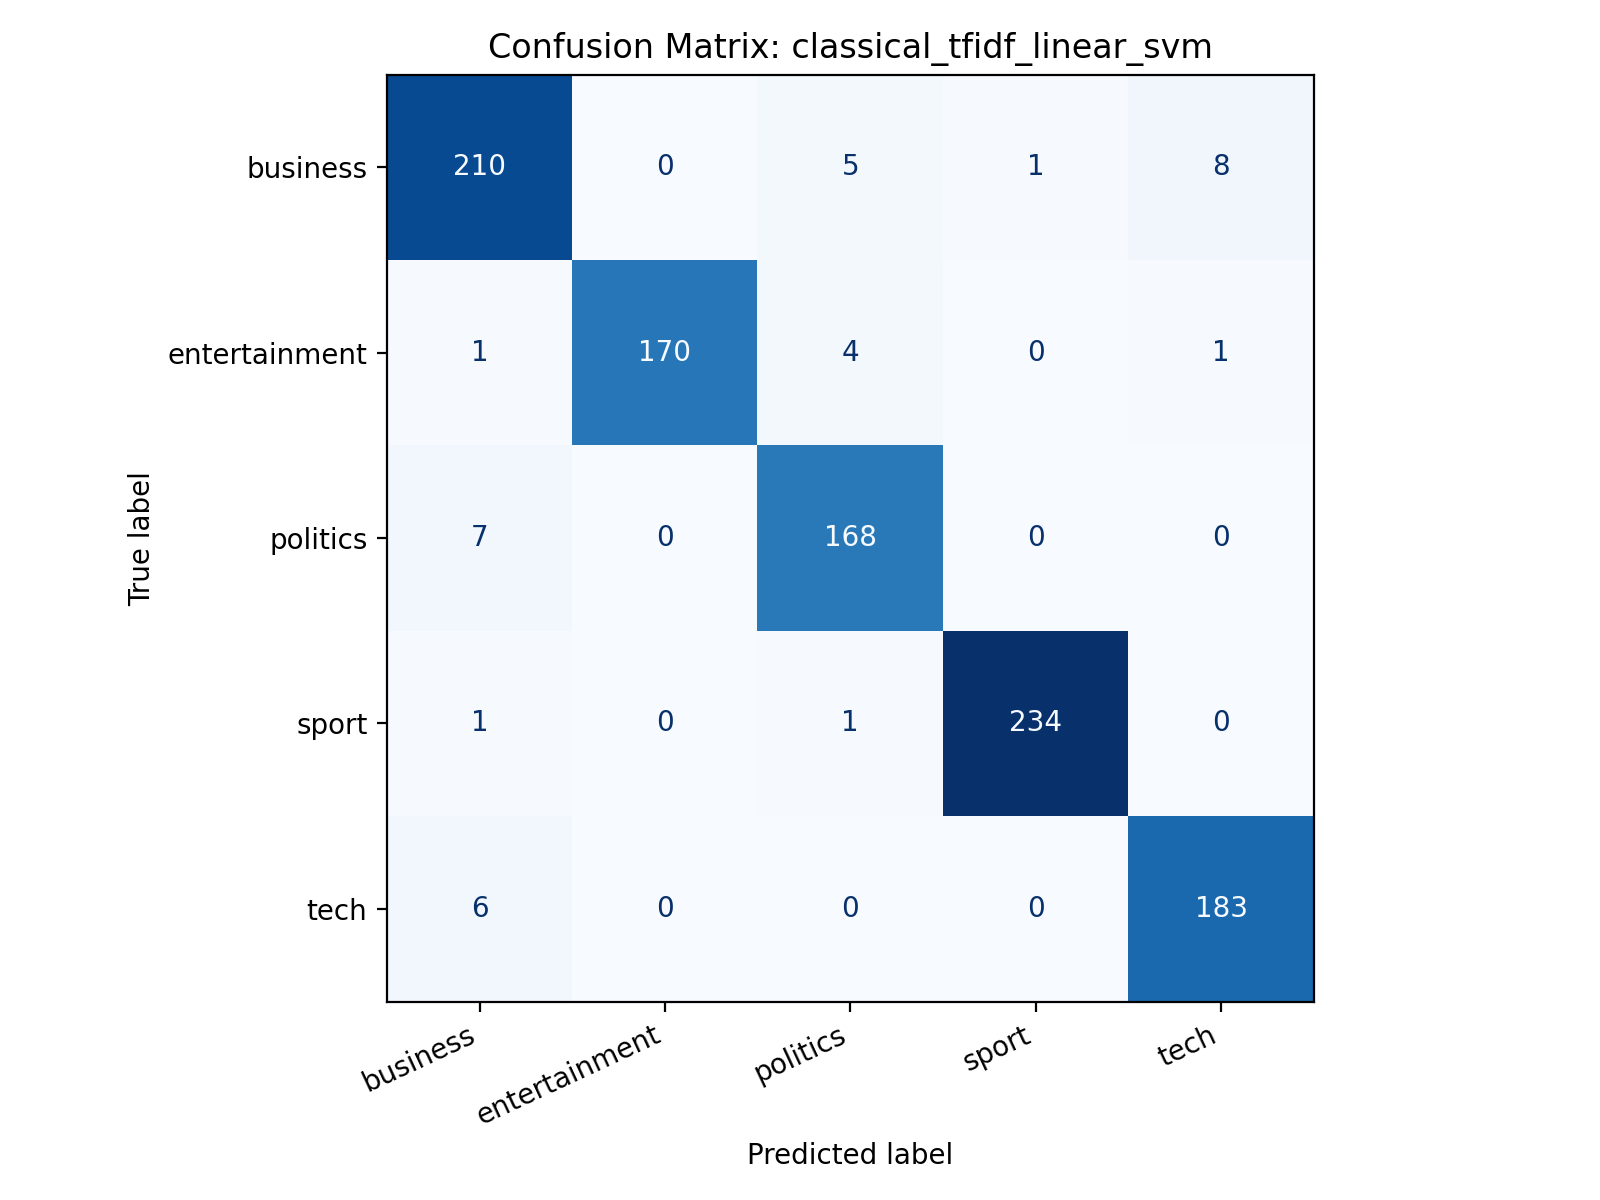
\includegraphics[width=\linewidth]{results_final_all/classification/confusion_matrices/classical_tfidf_linear_svm_confusion_matrix.png}
    \caption{Best overall model}
\end{subfigure}
\hfill
\begin{subfigure}{0.49\textwidth}
    \centering
    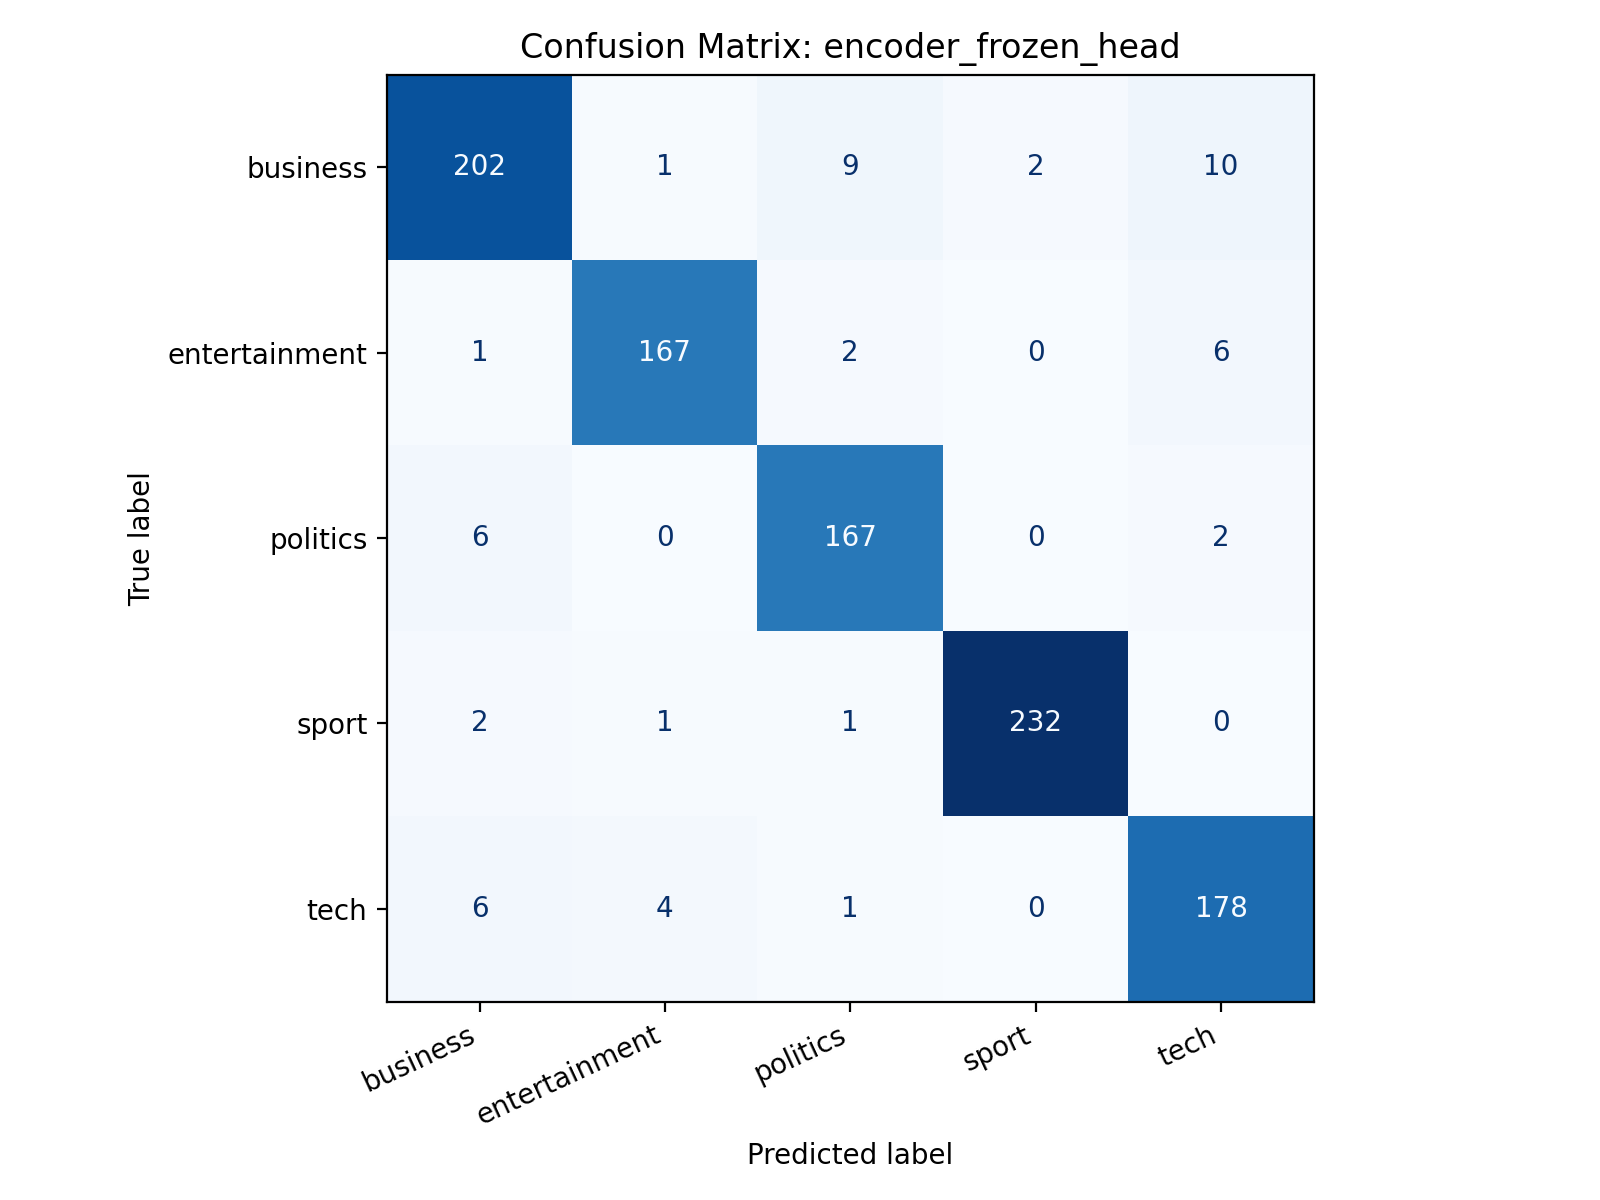
\includegraphics[width=\linewidth]{results_final_all/classification/confusion_matrices/encoder_frozen_head_confusion_matrix.png}
    \caption{Best transformer model}
\end{subfigure}
\caption{Confusion matrices for the strongest classical and encoder-based classifiers.}
\label{fig:classification-cm}
\end{figure}

The confusion matrices show that the strongest models classify most articles correctly, with remaining errors concentrated in semantically closer categories such as \texttt{business} versus \texttt{politics}, or \texttt{tech} versus \texttt{business}. These error patterns are intuitive because business and politics articles often share discussion of policy, regulation, or markets, while tech stories sometimes overlap with company news.

\subsection{Conclusion}

For classification, the best result came from a classical TF-IDF + Linear SVM model. The frozen encoder classifier was a close second and clearly outperformed zero-shot encoder similarity and both decoder-based approaches. The main lesson from Part 1 is that pretrained language models are highly effective, but a strong classical baseline remains difficult to beat on a small, lexically clean dataset like BBC News.

\section{Part 2: Clustering}

\subsection{Methodology}

For clustering, we followed the project instructions and compared three representations:

\begin{itemize}
\item encoder embeddings using the \texttt{[CLS]} token,
\item encoder embeddings using mean pooling over non-special tokens,
\item a classical TF-IDF representation.
\end{itemize}

For the encoder embeddings we used \texttt{sentence-transformers/all-MiniLM-L6-v2}. Clustering was performed with K-Means using $k=5$, matching the number of BBC categories. External validation used the ground-truth labels only after clustering. We report Adjusted Rand Index (ARI), Normalized Mutual Information (NMI), silhouette score, and runtime. To visualize clusters, we projected the representations to two dimensions with PCA.

We used the same encoder family for both \texttt{[CLS]} and mean-pooled document embeddings so that the only difference in the encoder-based clustering experiments is the pooling strategy. This makes the comparison cleaner and allows us to attribute quality differences directly to the representation rather than to a change in base model.

\subsection{Experimental Results \& Analysis}

\begin{table}[H]
\centering
\small
\caption{Clustering results on the BBC News test split.}
\label{tab:clustering}
\begin{tabular}{lcccc}
\toprule
Representation + Clustering & ARI & NMI & Silhouette & Runtime (s) \\
\midrule
Encoder [CLS] + K-Means & 0.7931 & 0.7584 & 0.0421 & 0.89 \\
Encoder mean pool + K-Means & \textbf{0.8756} & \textbf{0.8532} & \textbf{0.0517} & 0.89 \\
TF-IDF + K-Means & 0.4270 & 0.6244 & 0.0101 & 4.69 \\
\bottomrule
\end{tabular}
\end{table}

\begin{figure}[H]
\centering
\begin{subfigure}{0.49\textwidth}
    \centering
    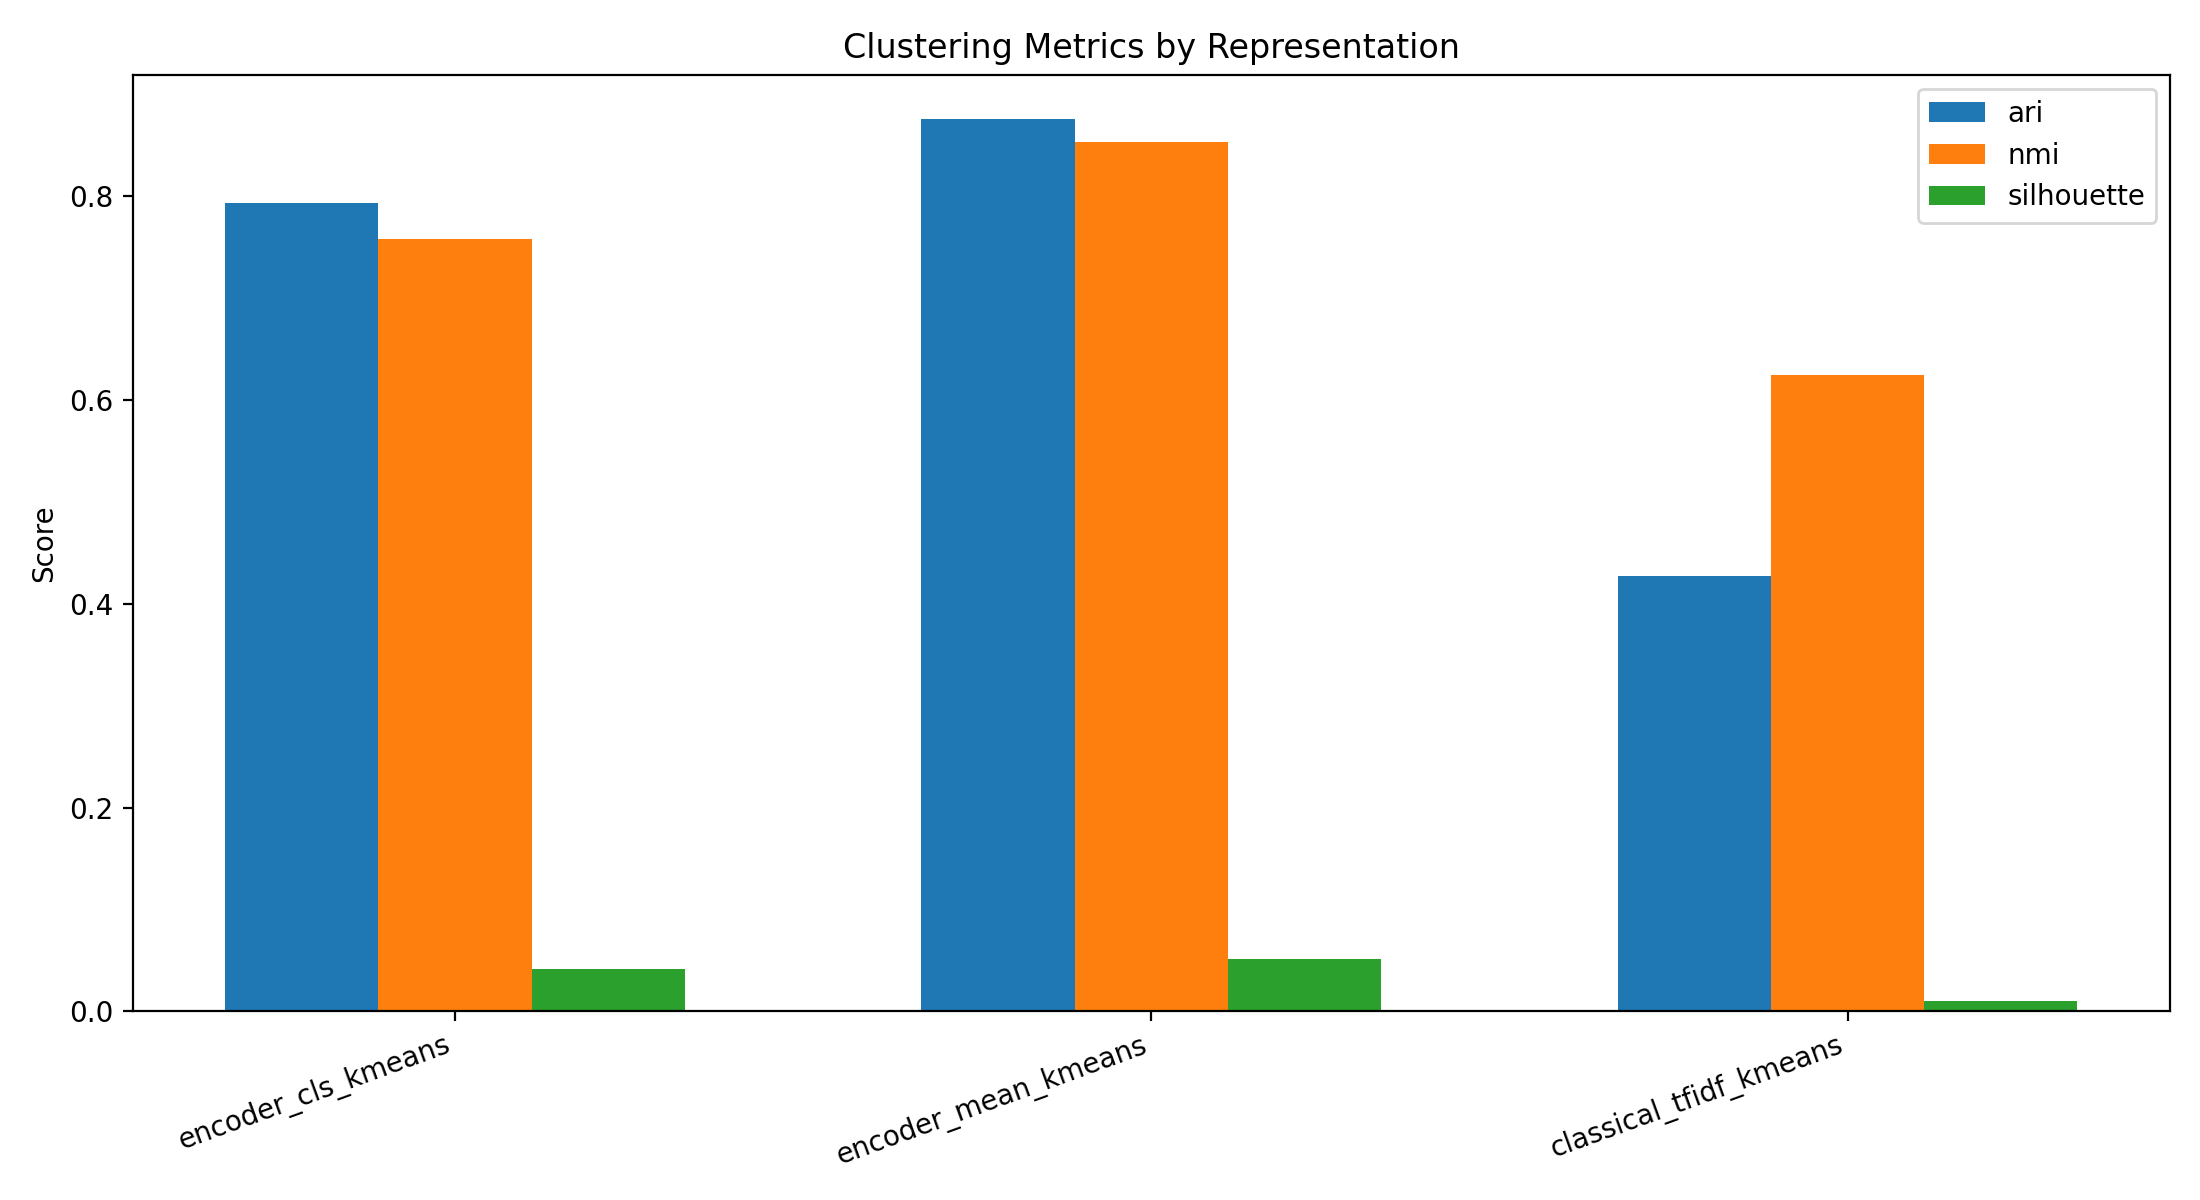
\includegraphics[width=\linewidth]{results_final_all/clustering/clustering_metrics.png}
    \caption{Clustering metric comparison}
\end{subfigure}
\hfill
\begin{subfigure}{0.49\textwidth}
    \centering
    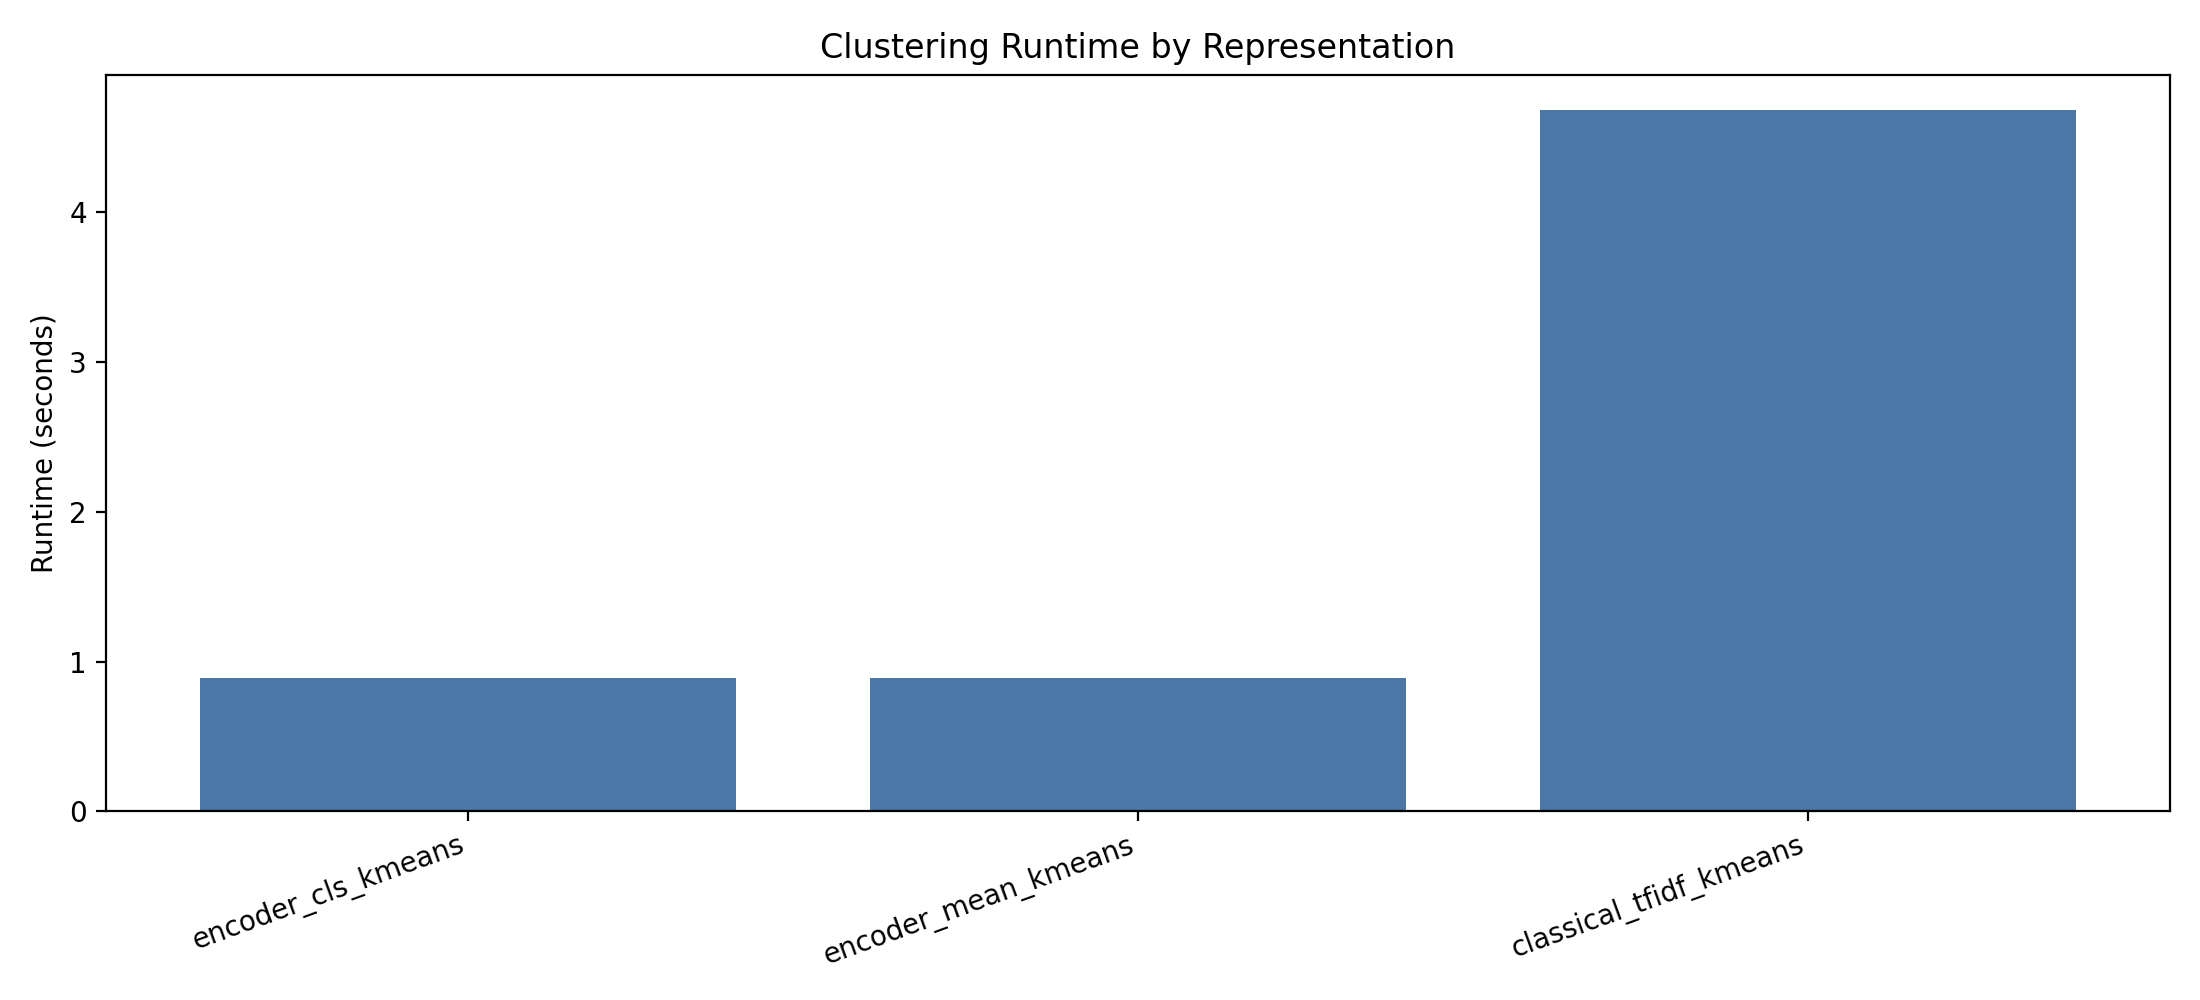
\includegraphics[width=\linewidth]{results_final_all/clustering/clustering_runtimes.png}
    \caption{Clustering runtime comparison}
\end{subfigure}
\caption{Summary plots for Part 2 clustering experiments.}
\label{fig:clustering-plots}
\end{figure}

The best clustering result came from encoder mean-pooled embeddings, which achieved ARI 0.8756 and NMI 0.8532. Encoder \texttt{[CLS]} embeddings were also strong, but mean pooling performed better on every reported metric. This is consistent with the intuition that mean pooling captures the article-level semantics more robustly than relying on a single token representation.

The classical TF-IDF clustering result was notably weaker, especially on ARI and silhouette score. This suggests that the encoder embedding space provides a more semantically organized representation for unsupervised grouping than sparse lexical counts alone. Another useful observation is runtime: even though TF-IDF is usually cheap for classification, in this clustering setup the TF-IDF K-Means pipeline was slower than the encoder clustering runs because of the dense conversion and clustering cost on the high-dimensional feature matrix.

The gap between encoder-based and classical clustering is larger than the gap observed in classification. This is an important result. In supervised classification, a classical linear model can use label information to compensate for a simpler representation. In clustering, however, there is no supervision to correct representation weaknesses. As a result, the quality of the feature space becomes much more important, and the semantic structure learned by the encoder clearly helps.

\begin{figure}[H]
\centering
\begin{subfigure}{0.48\textwidth}
    \centering
    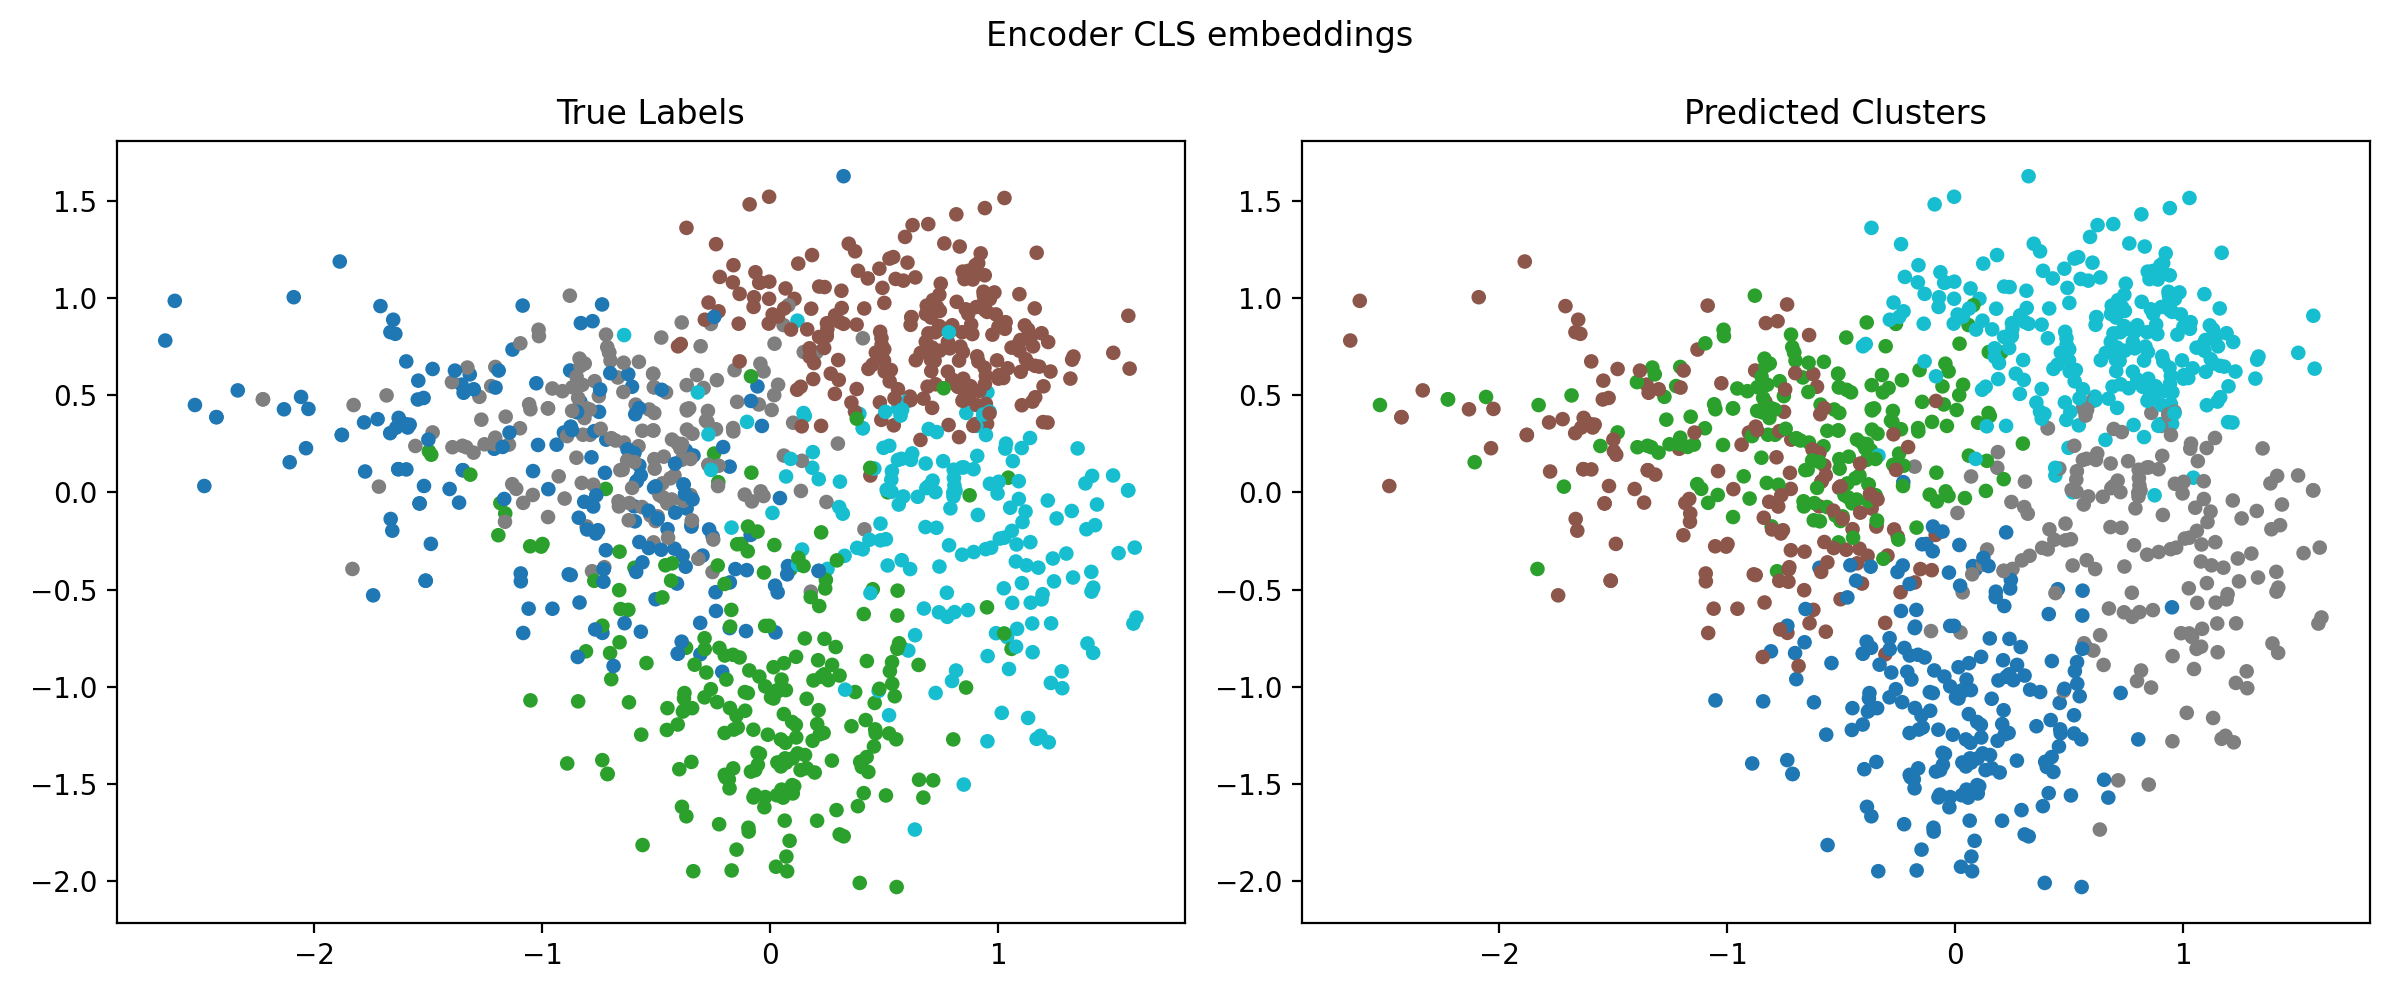
\includegraphics[width=\linewidth]{results_final_all/clustering/cluster_projection_cls.png}
    \caption{Encoder [CLS]}
\end{subfigure}
\hfill
\begin{subfigure}{0.48\textwidth}
    \centering
    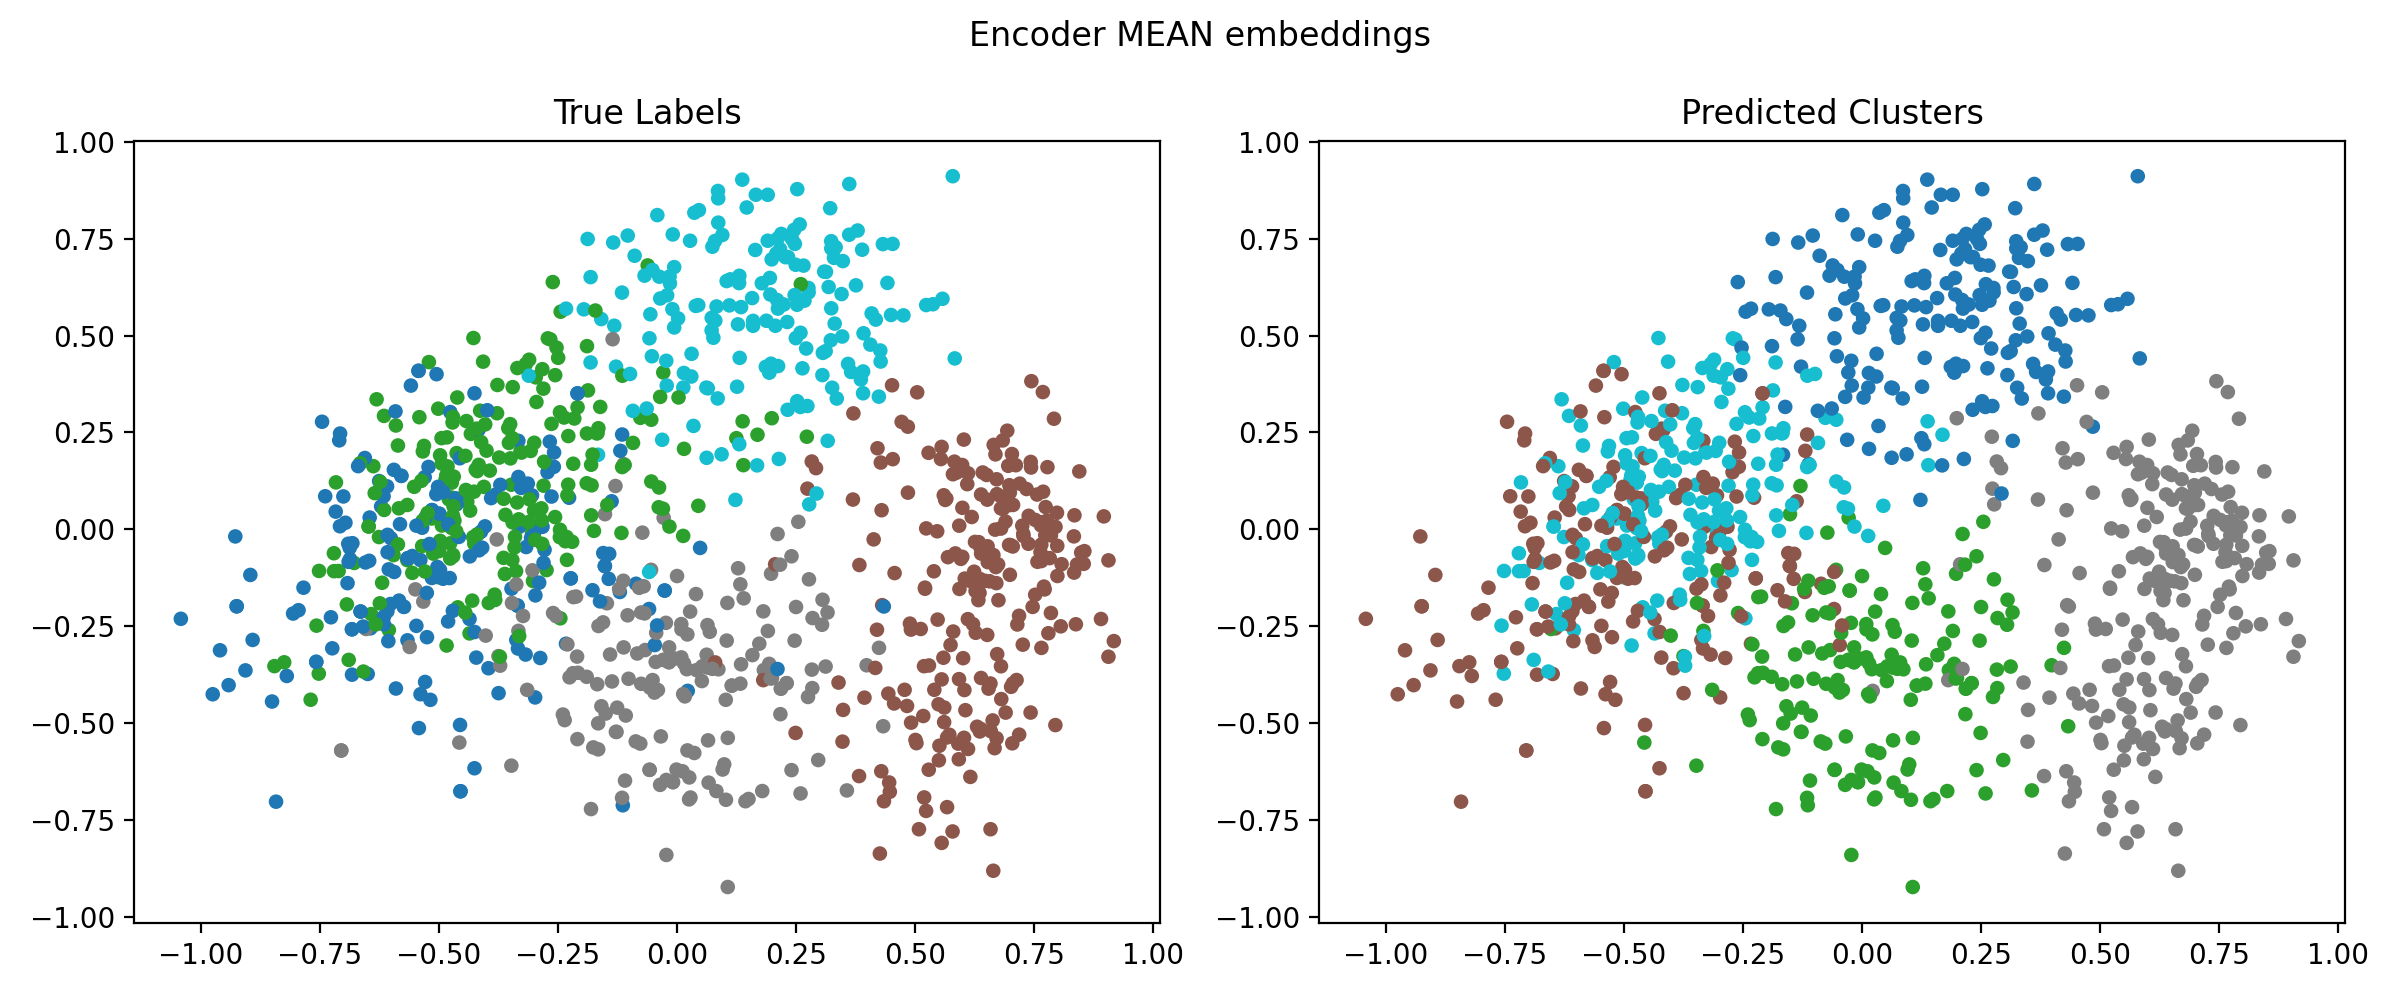
\includegraphics[width=\linewidth]{results_final_all/clustering/cluster_projection_mean.png}
    \caption{Encoder mean pool}
\end{subfigure}

\vspace{0.8em}

\begin{subfigure}{0.72\textwidth}
    \centering
    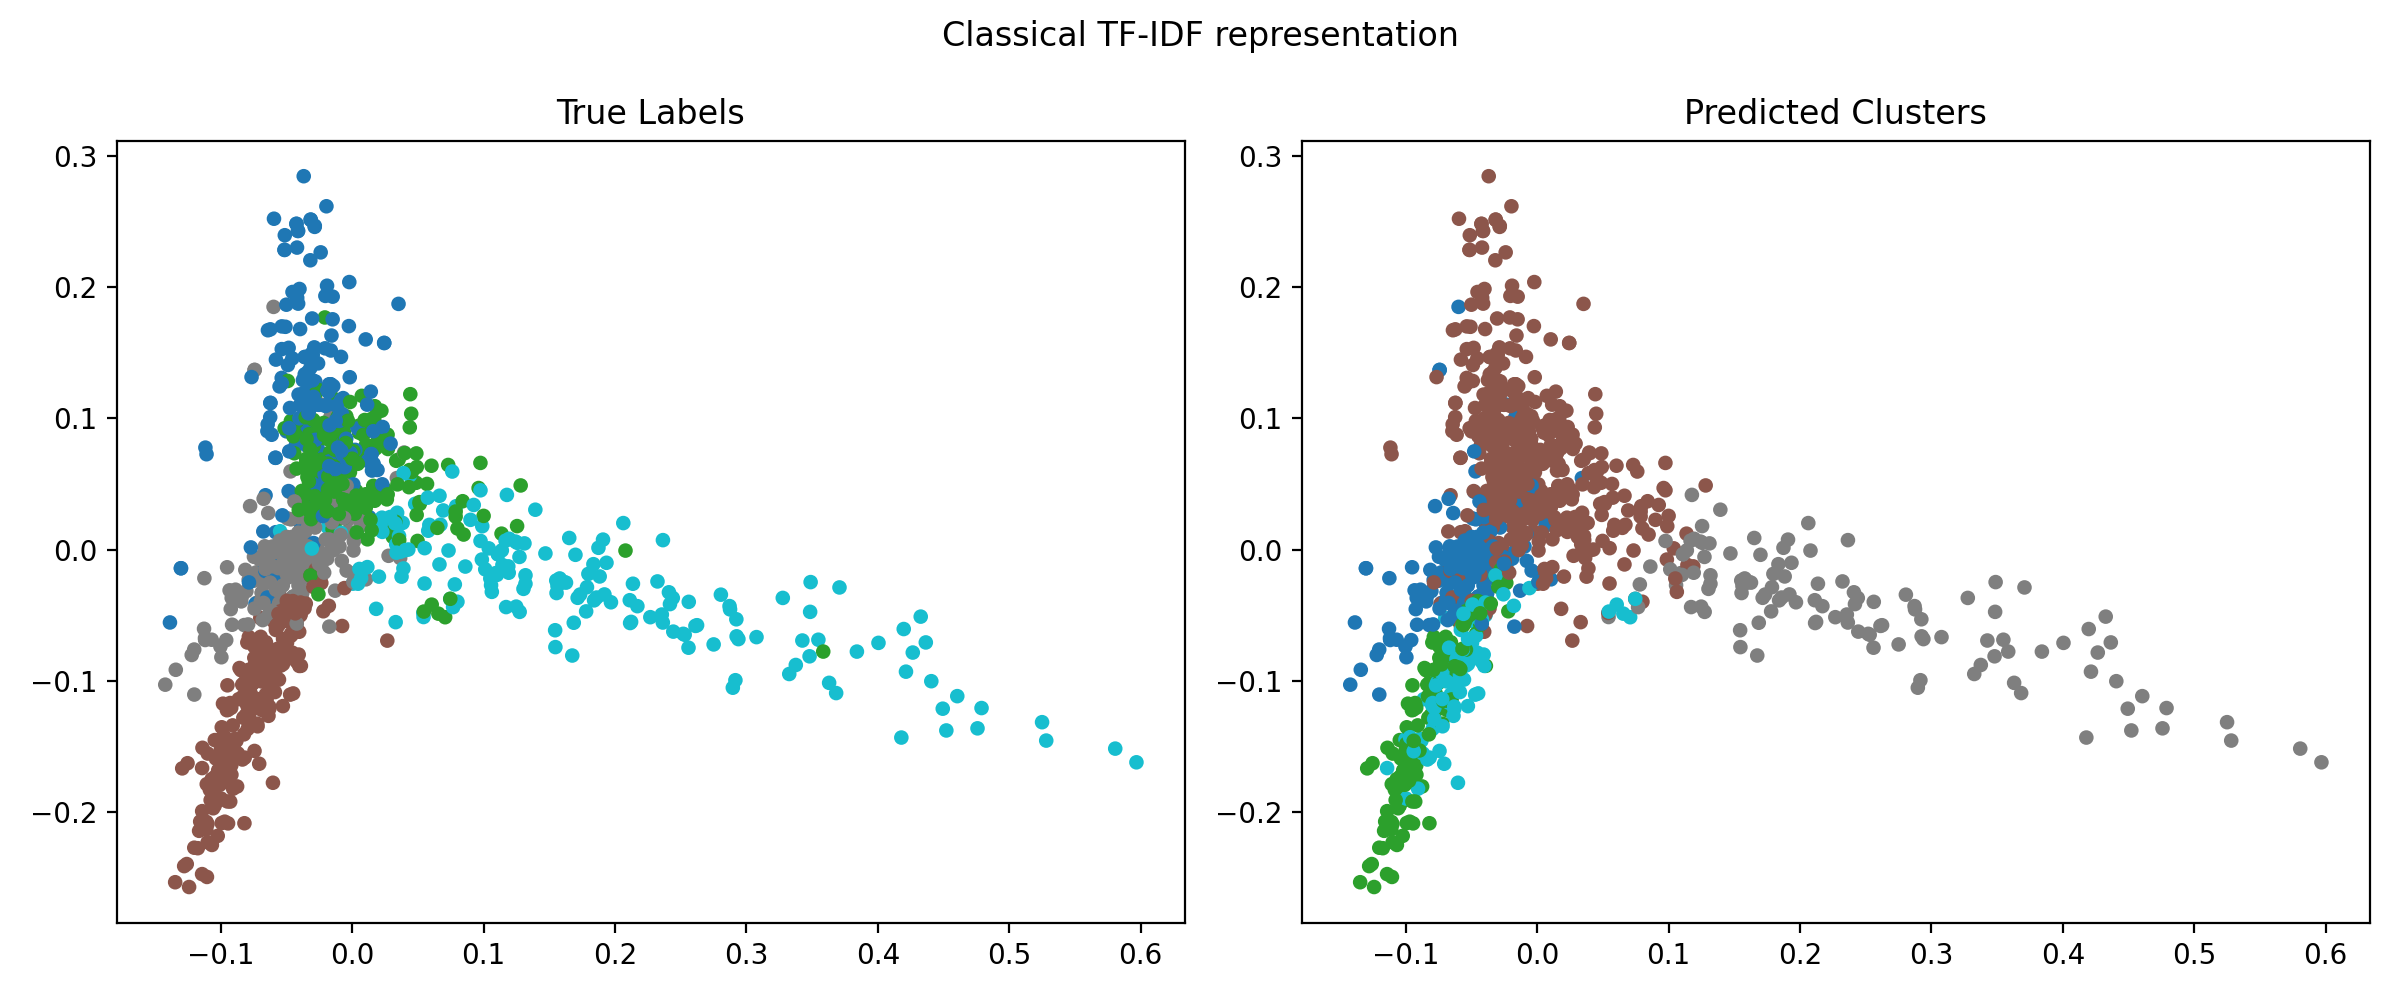
\includegraphics[width=\linewidth]{results_final_all/clustering/cluster_projection_tfidf.png}
    \caption{TF-IDF}
\end{subfigure}
\caption{Two-dimensional PCA projections of clustering outputs. The mean-pooled encoder representation shows the clearest separation.}
\label{fig:clustering-projections}
\end{figure}

The PCA projections visually support the quantitative results. The mean-pooled encoder representation forms more coherent groups, while TF-IDF produces more overlap between classes. The silhouette values are modest for all three methods because text clusters still overlap in semantic space, but the relative ranking remains consistent with ARI and NMI.

This consistency across multiple metrics is reassuring. ARI and NMI both favor the mean-pooled encoder representation, and the visualization points in the same direction. Even though the absolute silhouette values are not large, the relative ordering of methods is stable, which gives more confidence that the clustering conclusion is not an artifact of any single metric.

\subsection{Conclusion}

For clustering, encoder-derived embeddings were clearly better than the classical TF-IDF representation, and mean pooling outperformed \texttt{[CLS]} pooling. Part 2 shows that pretrained encoder representations are especially useful for unsupervised tasks because they capture semantic similarity directly, even without any supervised clustering objective.

\section{Overall Conclusion}

This project compared encoder models, decoder models, and classical text methods on both classification and clustering. The strongest classification result came from TF-IDF + Linear SVM, while the strongest clustering result came from mean-pooled encoder embeddings with K-Means. The encoder frozen-head classifier also performed very strongly, showing that pretrained encoders transfer well to classification with minimal task-specific training.

The most important lesson from this project is that different workflows are best suited to different tasks. Classical sparse models remain highly competitive for small supervised text classification problems, while pretrained encoder embeddings are especially strong for clustering and semantic grouping. Decoder-only models can perform classification through prompting, but they are slower and less accurate than encoder or classical alternatives in this setting.

From a learning perspective, this project was useful because it forced us to work with three very different paradigms inside one pipeline: traditional bag-of-words modeling, encoder-based representation learning, and decoder-based prompted inference. Seeing these approaches side by side made the tradeoffs much clearer. Overall, the project provided practical experience applying transformer-based language models to both classification and clustering, and reinforced the value of strong baselines, careful evaluation, and runtime-aware comparison.

\end{document}
